\documentclass{emulateapj}
%\documentclass[12pt,preprint]{aastex}

\usepackage{graphicx}
\usepackage{float}
\usepackage{amsmath}
\usepackage{epsfig,floatflt}



\begin{document}

\title{Project 4}

\author{Christer Dreierstad}

\email{chrisdre@student.matnat.uio.no}

\altaffiltext{1}{Institute of Physics, University of
  Oslo, P.O.\ Box 1029 Blindern, N-0315 Oslo, Norway}


%\date{Received - / Accepted -}

\begin{abstract}

\end{abstract}
\keywords{computational science: Ising model  --- methods: Metropolis, Monte Carlo}

\section{Introduction}
\label{sec:introduction}
To study the phase transitions of a magnetic system we consider the Ising model for a two-dimensional system with a finite lattice size. The particles (spins) that make up the crystal (lattice) can take two values representing spin up or down. The energy of the lattice can then, by the Ising model, be found by
%
\begin{gather*}
    E = -J\sum_{< kl >}^N s_k s_l,
\end{gather*}
%
when there is no external magnetic field applied to the system. The coupling constant J will be set to 1, which means we are studying a ferromagnetic interaction between the spins that make up the lattice. Since the coupling constant is dependent upon the material we study, setting this to 1 allows for a general model. For studying the phase transition we consider the  Metropolis algorithm, a Markov chain Monte Carlo method (MCMC). 

\section{Method}
\label{sec:method}
The two-dimensional binary Ising model has analytical expectation values. The partition function
%
\begin{equation*}
    z = \sum_i \Omega(E_i) e^{\beta E_i},
\end{equation*}
%
where $\Omega(E_i)$ is the degeneracy of energy $E_i$ and $\beta = 1/k_BT$. From Table \ref{tab:energies} we can see that there are 2 energies that are non-zero: $\pm 8J$, which both has a degeneracy of 2. The energy equal to zero has a degeneracy of 12. Expanding the sum of the partition function we get 
%
\begin{align*}
    z &= 2e^{8J\beta} + 12 + 2e^{-8J\beta} \\
    &= 12 + 2\left(e^{8J\beta} + e^{-8J\beta}\right),
\end{align*}
%
where we have inserted $e^0 = 1$. We know that $\cosh(x) = \frac{1}{2}\left( e^{-x} + e^x\right)$, inserting this gives
%
\begin{gather}\label{eq:z}
    Z = 12 + 4\cosh(8J\beta).
\end{gather}
%
The mean value of the energy is given by
%
\begin{align*}
    \langle E \rangle = -\frac{\partial }{\partial \beta} \ln Z = -\frac{1}{Z}\frac{\partial Z}{\partial \beta},
\end{align*}
%
which is found by inserting the partition function.
%
\begin{align*}
    \langle E \rangle &= -\frac{1}{Z}\frac{\partial}{\partial \beta} \left(12 + 4 \cosh\left(8J\beta\right)\right)\\
    &= -\frac{4}{Z}\left(8J\sinh\left(8J\beta\right)\right),
\end{align*}
pulling a factor 4 from the partition function and inserting we are left with a analytical solution to the mean energy of the lattice
%
\begin{gather*}
    \langle E \rangle = -\frac{8J\sinh\left(8J\beta\right)}{3 + \cosh(8J\beta}.
\end{gather*}
%
The heat capacity can be found by
%
\begin{align*}
    C_V &= \frac{1}{kT^2}\frac{\partial^2}{\partial \beta^2} \ln Z = \frac{1}{kT^2}\frac{\partial}{\partial \beta}\left(\frac{\partial}{\partial \beta} \ln Z\right),
\end{align*}
%
where we recognize the partial derivative in the parenthesis as the negative mean energy. 
%
\begin{align*}
    C_V = \frac{1}{kT^2}&\left(\frac{64J^2\cosh\left(8J\beta\right)\left(3 + \cosh\left(8J\beta\right)\right)}{\left(3 + \cosh\left(8J\beta\right)\right)^2}\right \\
    &-\left \frac{64J^2\sinh^2\left(8J\beta\right)}{\left(3 + \cosh\left(8J\beta\right)\right)^2}\right),
\end{align*}
%
by inserting for the mean energy and using the product rule. Further simplifications gives the mean heat capacity
%
\begin{gather*}
    C_V = \frac{1}{kT^2}\frac{64\cosh\left(8J\beta\right)}{ 3 + \cosh\left(8J\beta\right)}.
\end{gather*}
The susceptibility is given as
%
\begin{equation*}
    \chi = \frac{1}{kT}\left(\langle M^2 \rangle - \langle M \rangle^2\right).
\end{equation*}
%
To find the susceptibility of the system we consider the mean magnetic moment
%
\begin{equation*}
    \langle M \rangle = \frac{1}{Z} \sum_i |M_i| e^{-\beta E_i},
\end{equation*}
where we find the magnetic moment for a given energy in Table \ref{tab:energies}. So the mean magnetic moment is
%
\begin{equation*}
    \langle M \rangle = \frac{1}{Z}\left(4e^{8J\beta} + 4\left(2e^{0}\right) + 4\left(-2e^0\right) + -4e^{8J\beta} \right) = 0.
\end{equation*}
%
Further we calculate the mean of the  magnetic moment squared
%
\begin{equation*}
    \langle M^2 \rangle = \frac{1}{Z}\sum_i M_i^2 e^{-\beta E_i},
\end{equation*}
and again referring to Table \ref{tab:energies} we get
%
\begin{align*}
    \langle M^2 \rangle &= \frac{1}{Z}\left(16\left(2e^{8J\beta}\right) + 16\left(2e^0\right) \right) \\
    &= \frac{8\left(e^{8J\beta} + 1\right)}{3 + \cosh\left(8J\beta\right)}.
\end{align*}
So the susceptibility of the system is given as
%
\begin{equation*}
    \chi = \frac{1}{kT^2}\langle M^2 \rangle = \frac{1}{kT^2}\frac{8\left(e^{8J\beta} + 1\right)}{3 + \cosh\left(8J\beta\right)}
\end{equation*}
%
Further we find the mean of the absolute value of the magnetic moment by

\begin{align*}
    \langle |M| \rangle &= \frac{1}{Z} \sum_i |M_i| e^{-\beta E_i} \\
     &= \frac{1}{Z}\left(4e^{8J\beta} + 4\left(2e^{0}\right) + 4\left(|-2|e^0\right) + |-4|e^{8J\beta} \right) \\
     &= \frac{2e^{8J\beta} + 4}{3 + \cosh\left(8J\beta\right)},
\end{align*}
%
after pulling out a factor 4 from the partition function. To summarize we have the following analytical expression for the system
%
\begin{align*}
    \langle E \rangle &= -\frac{4}{Z}\left(8J\sinh\left(8J\beta\right)\right), \\
    \langle |M| \rangle &= \frac{2e^{8J\beta} + 4}{3 + \cosh\left(8J\beta\right)}, \\
    C_V &= \frac{1}{kT^2}\frac{64\cosh\left(8J\beta\right)}{ 3 + \cosh\left(8J\beta\right)}, \\
    \chi &= \frac{1}{kT^2}\frac{8\left(e^{8J\beta} + 1\right)}{3 + \cosh\left(8J\beta\right)}.
\end{align*}


\begin{deluxetable}{cccc}
\tablewidth{0pt}
\tablecaption{\label{tab:energies}}
\tablecomments{...}
\tablecolumns{4}
\tablehead{Spins up  & Degeneracy & Energy & Magnetic moment}
\startdata
4 & 1 & -8J & 4 \\
3 & 4 & 0 & 2 \\
2 & 4 & 0 & 0 \\
2 & 2 & 8J & 0 \\
1 & 4 & 0 & -2 \\
0 & 1 & -8J & -4
\enddata
\end{deluxetable}


\section{Results}
\label{sec:results}

\begin{figure}[H]
{{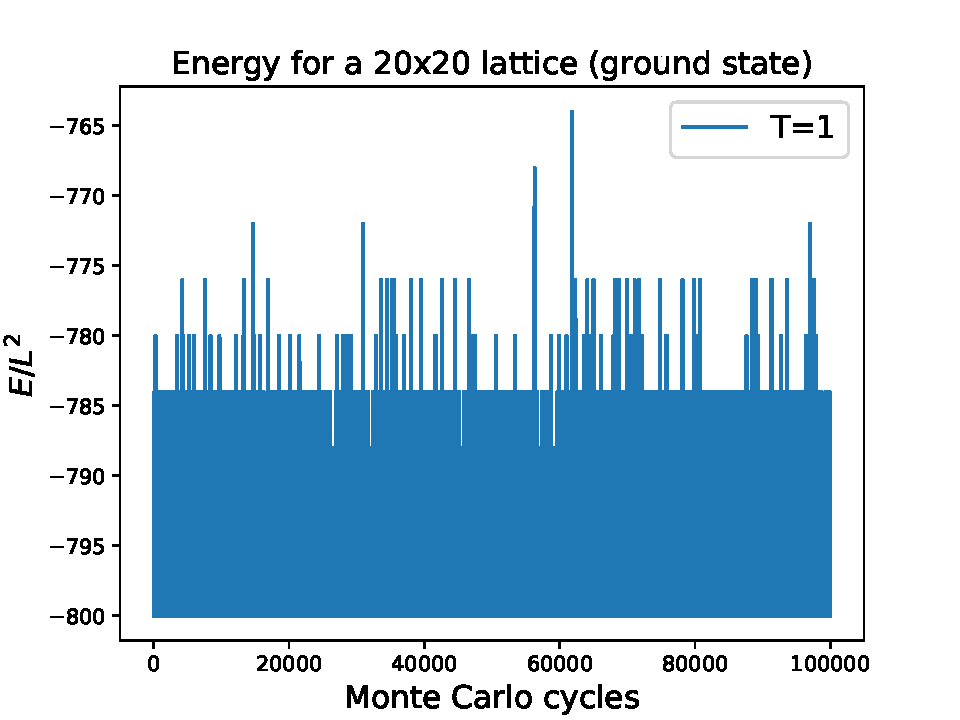
\includegraphics[scale=0.53]{EofMCC-GS-T1-L20-1e5.pdf}}
\subfloat{(a) hva skjer}
}\qquad
{{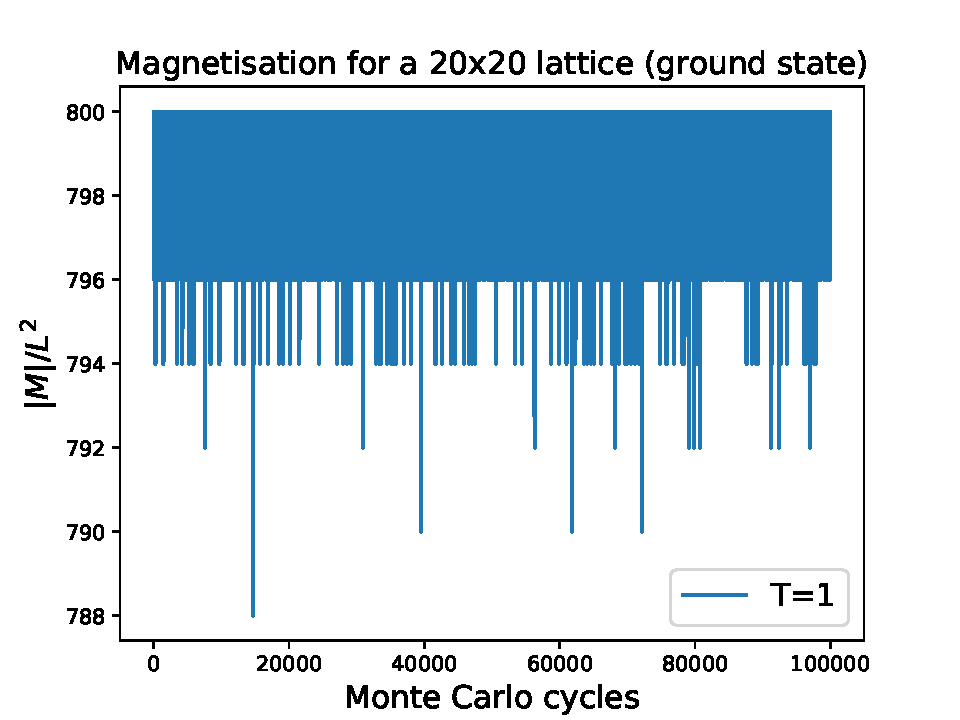
\includegraphics[scale=0.53]{MofMCC-GS-T1-L20-1e5.pdf}}
\subfloat{(b) }
}\qquad
\caption{text}
\label{fig:GS}
\end{figure}

\begin{figure}[H]
{{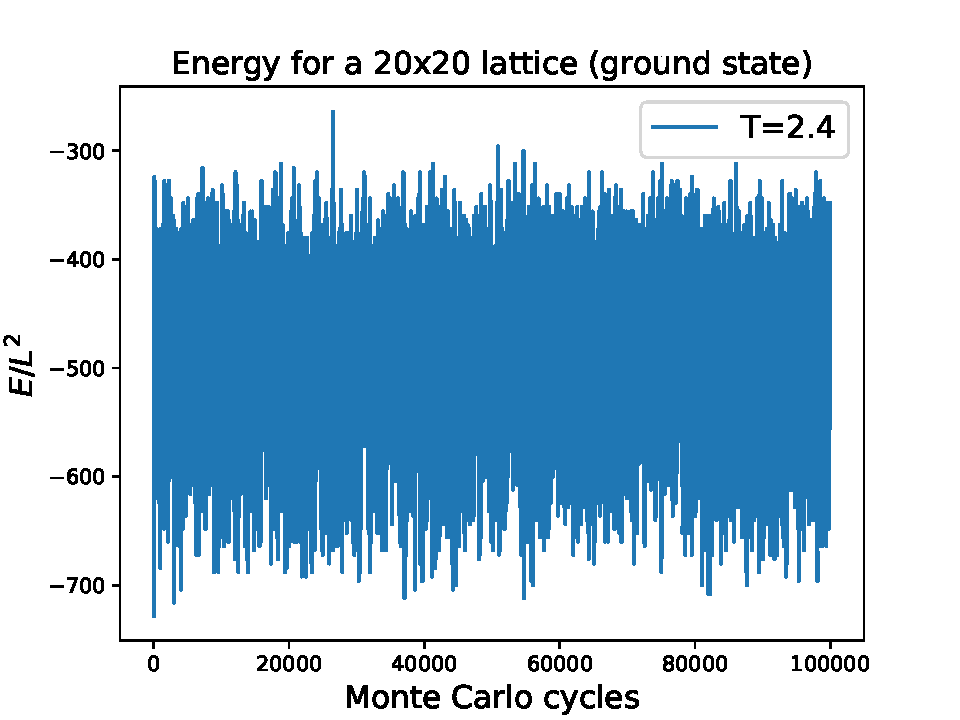
\includegraphics[scale=0.53]{EofMCC-GS-T2_4-L20-1e5.pdf}}
\subfloat{(a) }
}\qquad
{{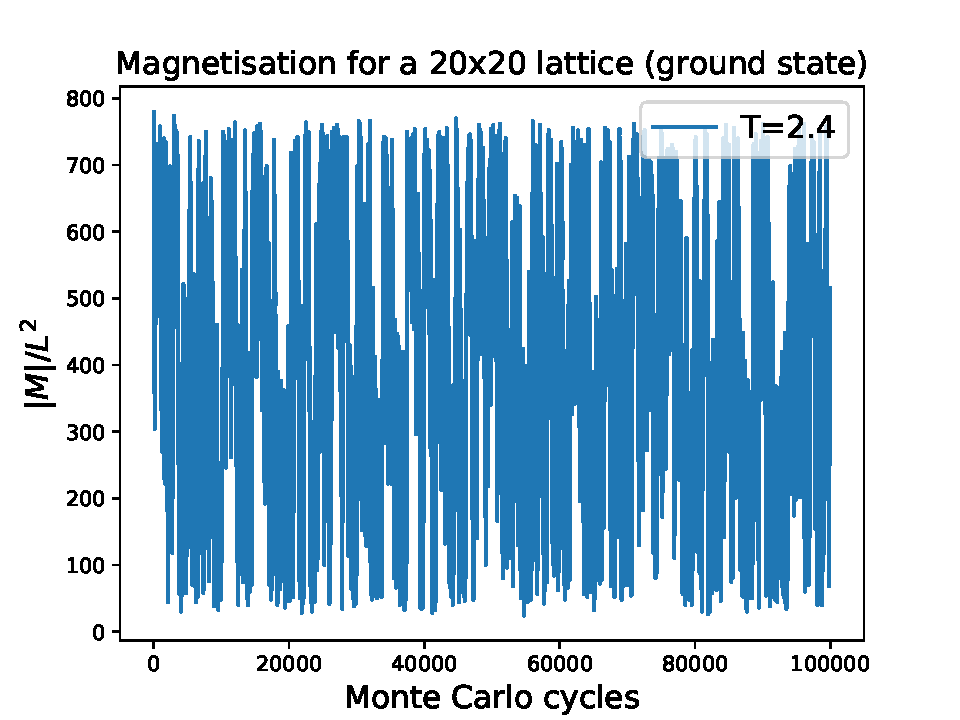
\includegraphics[scale=0.53]{MofMCC-GS-T2_4-L20-1e5.pdf}}
\subfloat{(b) }
}\qquad
\caption{text}
\label{fig:GS}
\end{figure}

\begin{figure}[H]
{{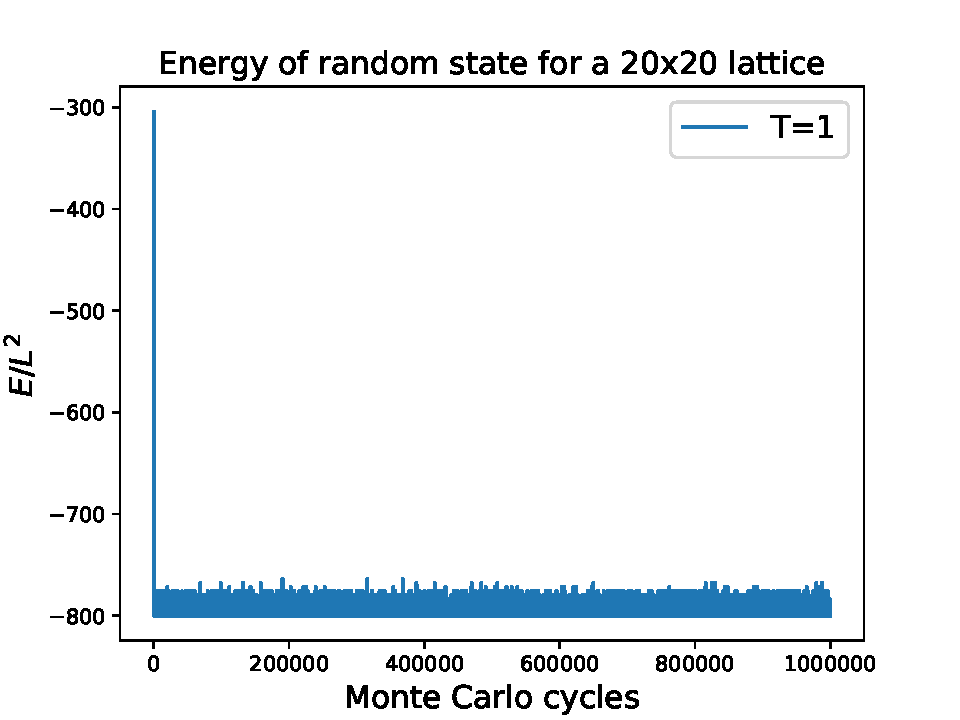
\includegraphics[scale=0.53]{EofMCC-T1-L20-1e6.pdf}}
\subfloat{(a) }
}\qquad
{{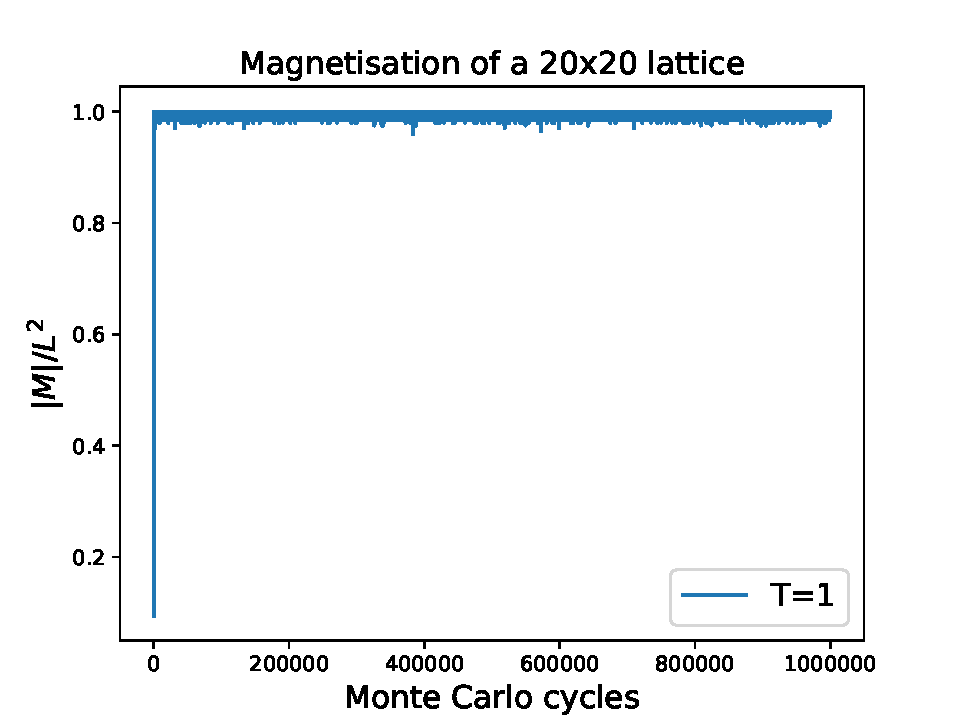
\includegraphics[scale=0.53]{MofMCC-T1-L20-1e6.pdf.pdf}}
\subfloat{(b) }
}\qquad
\caption{text}
\label{fig:GS}
\end{figure}

\begin{figure}[H]
{{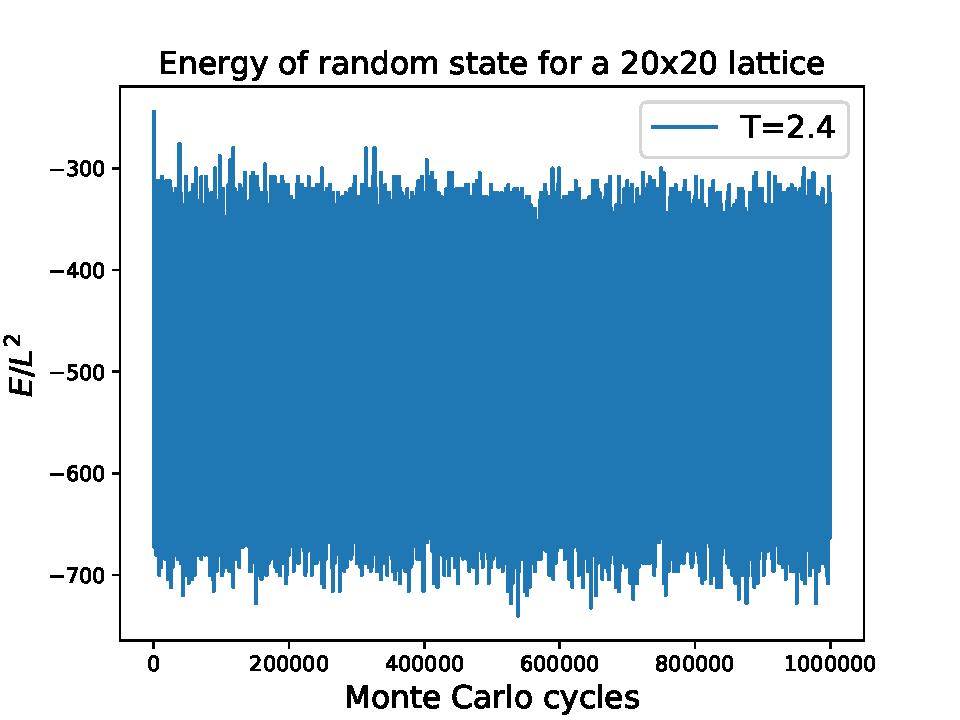
\includegraphics[scale=0.53]{EofMCC-T2_4-L20-1e6.pdf}}
\subfloat{(b) }
}\qquad
{{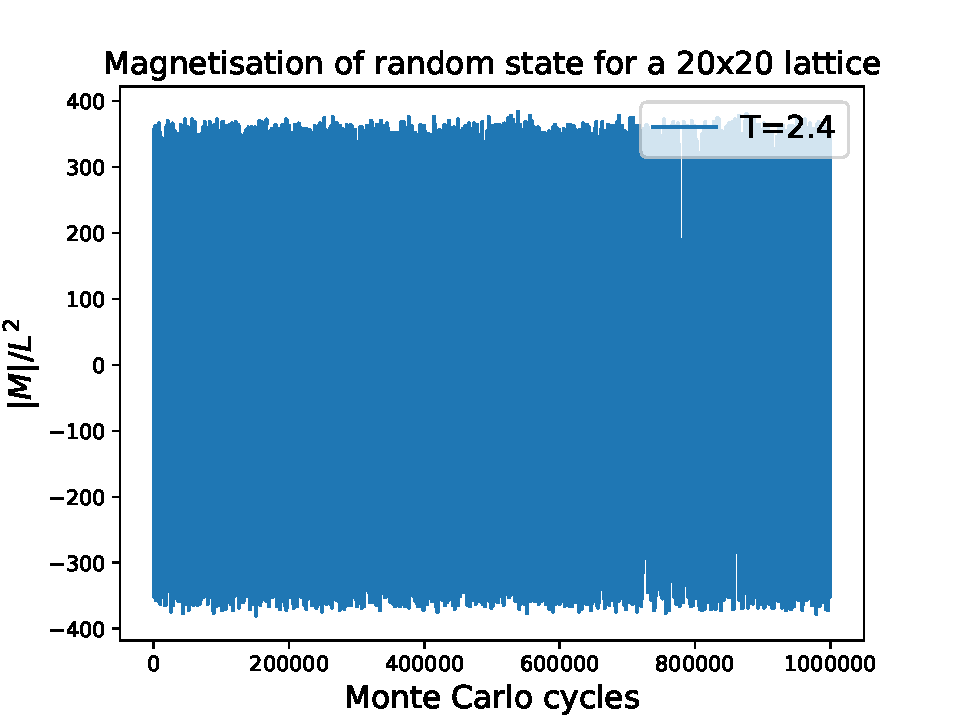
\includegraphics[scale=0.53]{MofMCC-T2_4-L20-1e6.pdf}}
\subfloat{(c) }
}\qquad
\caption{text}
\label{fig:GS}
\end{figure}

\begin{figure}[t]
\mbox{\epsfig{figure=accepts_of_T-T1T2_4-L20.pdf,width=\linewidth,clip=}}
\caption{Description of figure -- explain all elements, but do not
draw conclusions here.}
\label{fig:figure_label}
\end{figure}

\begin{figure}[t]
\mbox{\epsfig{figure=accepts-T1T2_4-L20-1e5.pdf,width=\linewidth,clip=}}
\caption{Description of figure -- explain all elements, but do not
draw conclusions here.}
\label{fig:figure_label}
\end{figure}

\begin{figure}[t]
\mbox{\epsfig{figure=CV-T2-23.pdf,width=\linewidth,clip=}}
\caption{Description of figure -- explain all elements, but do not
draw conclusions here.}
\label{fig:figure_label}
\end{figure}

\begin{figure}[t]
\mbox{\epsfig{figure=CV-T2-23.pdf,width=\linewidth,clip=}}
\caption{Description of figure -- explain all elements, but do not
draw conclusions here.}
\label{fig:figure_label}
\end{figure}

\begin{figure}[t]
\mbox{\epsfig{figure=CV-T22-24.pdf,width=\linewidth,clip=}}
\caption{Description of figure -- explain all elements, but do not
draw conclusions here.}
\label{fig:figure_label}
\end{figure}

\begin{figure}[t]
\mbox{\epsfig{figure=E-T2-23.pdf,width=\linewidth,clip=}}
\caption{Description of figure -- explain all elements, but do not
draw conclusions here.}
\label{fig:figure_label}
\end{figure}

\begin{figure}[t]
\mbox{\epsfig{figure=E-T22-24.pdf,width=\linewidth,clip=}}
\caption{Description of figure -- explain all elements, but do not
draw conclusions here.}
\label{fig:figure_label}
\end{figure}

\begin{figure}[t]
\mbox{\epsfig{figure=FittedTc.pdf,width=\linewidth,clip=}}
\caption{Description of figure -- explain all elements, but do not
draw conclusions here.}
\label{fig:figure_label}
\end{figure}

\begin{figure}[t]
\mbox{\epsfig{figure=M-T2-23.pdf,width=\linewidth,clip=}}
\caption{Description of figure -- explain all elements, but do not
draw conclusions here.}
\label{fig:figure_label}
\end{figure}

\begin{figure}[t]
\mbox{\epsfig{figure=M-T22-24.pdf,width=\linewidth,clip=}}
\caption{Description of figure -- explain all elements, but do not
draw conclusions here.}
\label{fig:figure_label}
\end{figure}

\begin{figure}[t]
\mbox{\epsfig{figure=PE-T1-L20-1e6.pdf,width=\linewidth,clip=}}
\caption{Description of figure -- explain all elements, but do not
draw conclusions here.}
\label{fig:figure_label}
\end{figure}


\begin{figure}[t]
\mbox{\epsfig{figure=PE-T2_4-L20-1e6.pdf,width=\linewidth,clip=}}
\caption{Description of figure -- explain all elements, but do not
draw conclusions here.}
\label{fig:figure_label}
\end{figure}


\begin{figure}[t]
\mbox{\epsfig{figure=X-T2-23.pdf,width=\linewidth,clip=}}
\caption{Description of figure -- explain all elements, but do not
draw conclusions here.}
\label{fig:figure_label}
\end{figure}

\begin{figure}[t]
\mbox{\epsfig{figure=X-T22-24.pdf,width=\linewidth,clip=}}
\caption{Description of figure -- explain all elements, but do not
draw conclusions here.}
\label{fig:figure_label}
\end{figure}





\section{Discussion}
\label{sec:discussion}




\section{Conclusions}
\label{sec:conclusions}




%\begin{figure}[t]
%
%\mbox{\epsfig{figure=filename.eps,width=\linewidth,clip=}}
%
%\caption{Description of figure -- explain all elements, but do not
%draw conclusions here.}
%\label{fig:figure_label}
%\end{figure}



%\begin{deluxetable}{lccc}
%\tablewidth{0pt}
%\tablecaption{\label{tab:results}}
%\tablecomments{Summary of main results.}
%\tablecolumns{4}
%\tablehead{Column 1  & Column 2 & Column 3 & Column 4}
%\startdata
%Item 1 & Item 2 & Item 3 & Item 4
%\enddata
%\end{deluxetable}



\begin{acknowledgements}

\end{acknowledgements}

\begin{thebibliography}{}

\bibitem[G{\'o}rski et al.(1994)]{gorski:1994} G{\'o}rski, K. M.,
  Hinshaw, G., Banday, A. J., Bennett, C. L., Wright, E. L., Kogut,
  A., Smoot, G. F., and Lubin, P.\ 1994, ApJL, 430, 89

\end{thebibliography}


\end{document}
